\section{Context}

This research is the latest on a long line of academic articles on the topics of retrieval-augmented generation, counterparametric and contextual data, and how to enhance knowledge on large language models.

This section summarizes key articles that informed this research.

\subsection{Foundational Papers on Large Language Models}

Large language models have exploded in popularity since the development of the transformer architecture \citep{attention_is_all_you_need}.
This architecture relies entirely on self-attention mechanisms rather than recurrent or convolutional layers, which allow the model to weigh the importance of different words in a sequence relative to each other, irrespective of their position.
This mechanism enables the model to capture complex dependencies and relationships across long sequences more effectively than traditional models.

\begin{figure}[htb]
	\centering
	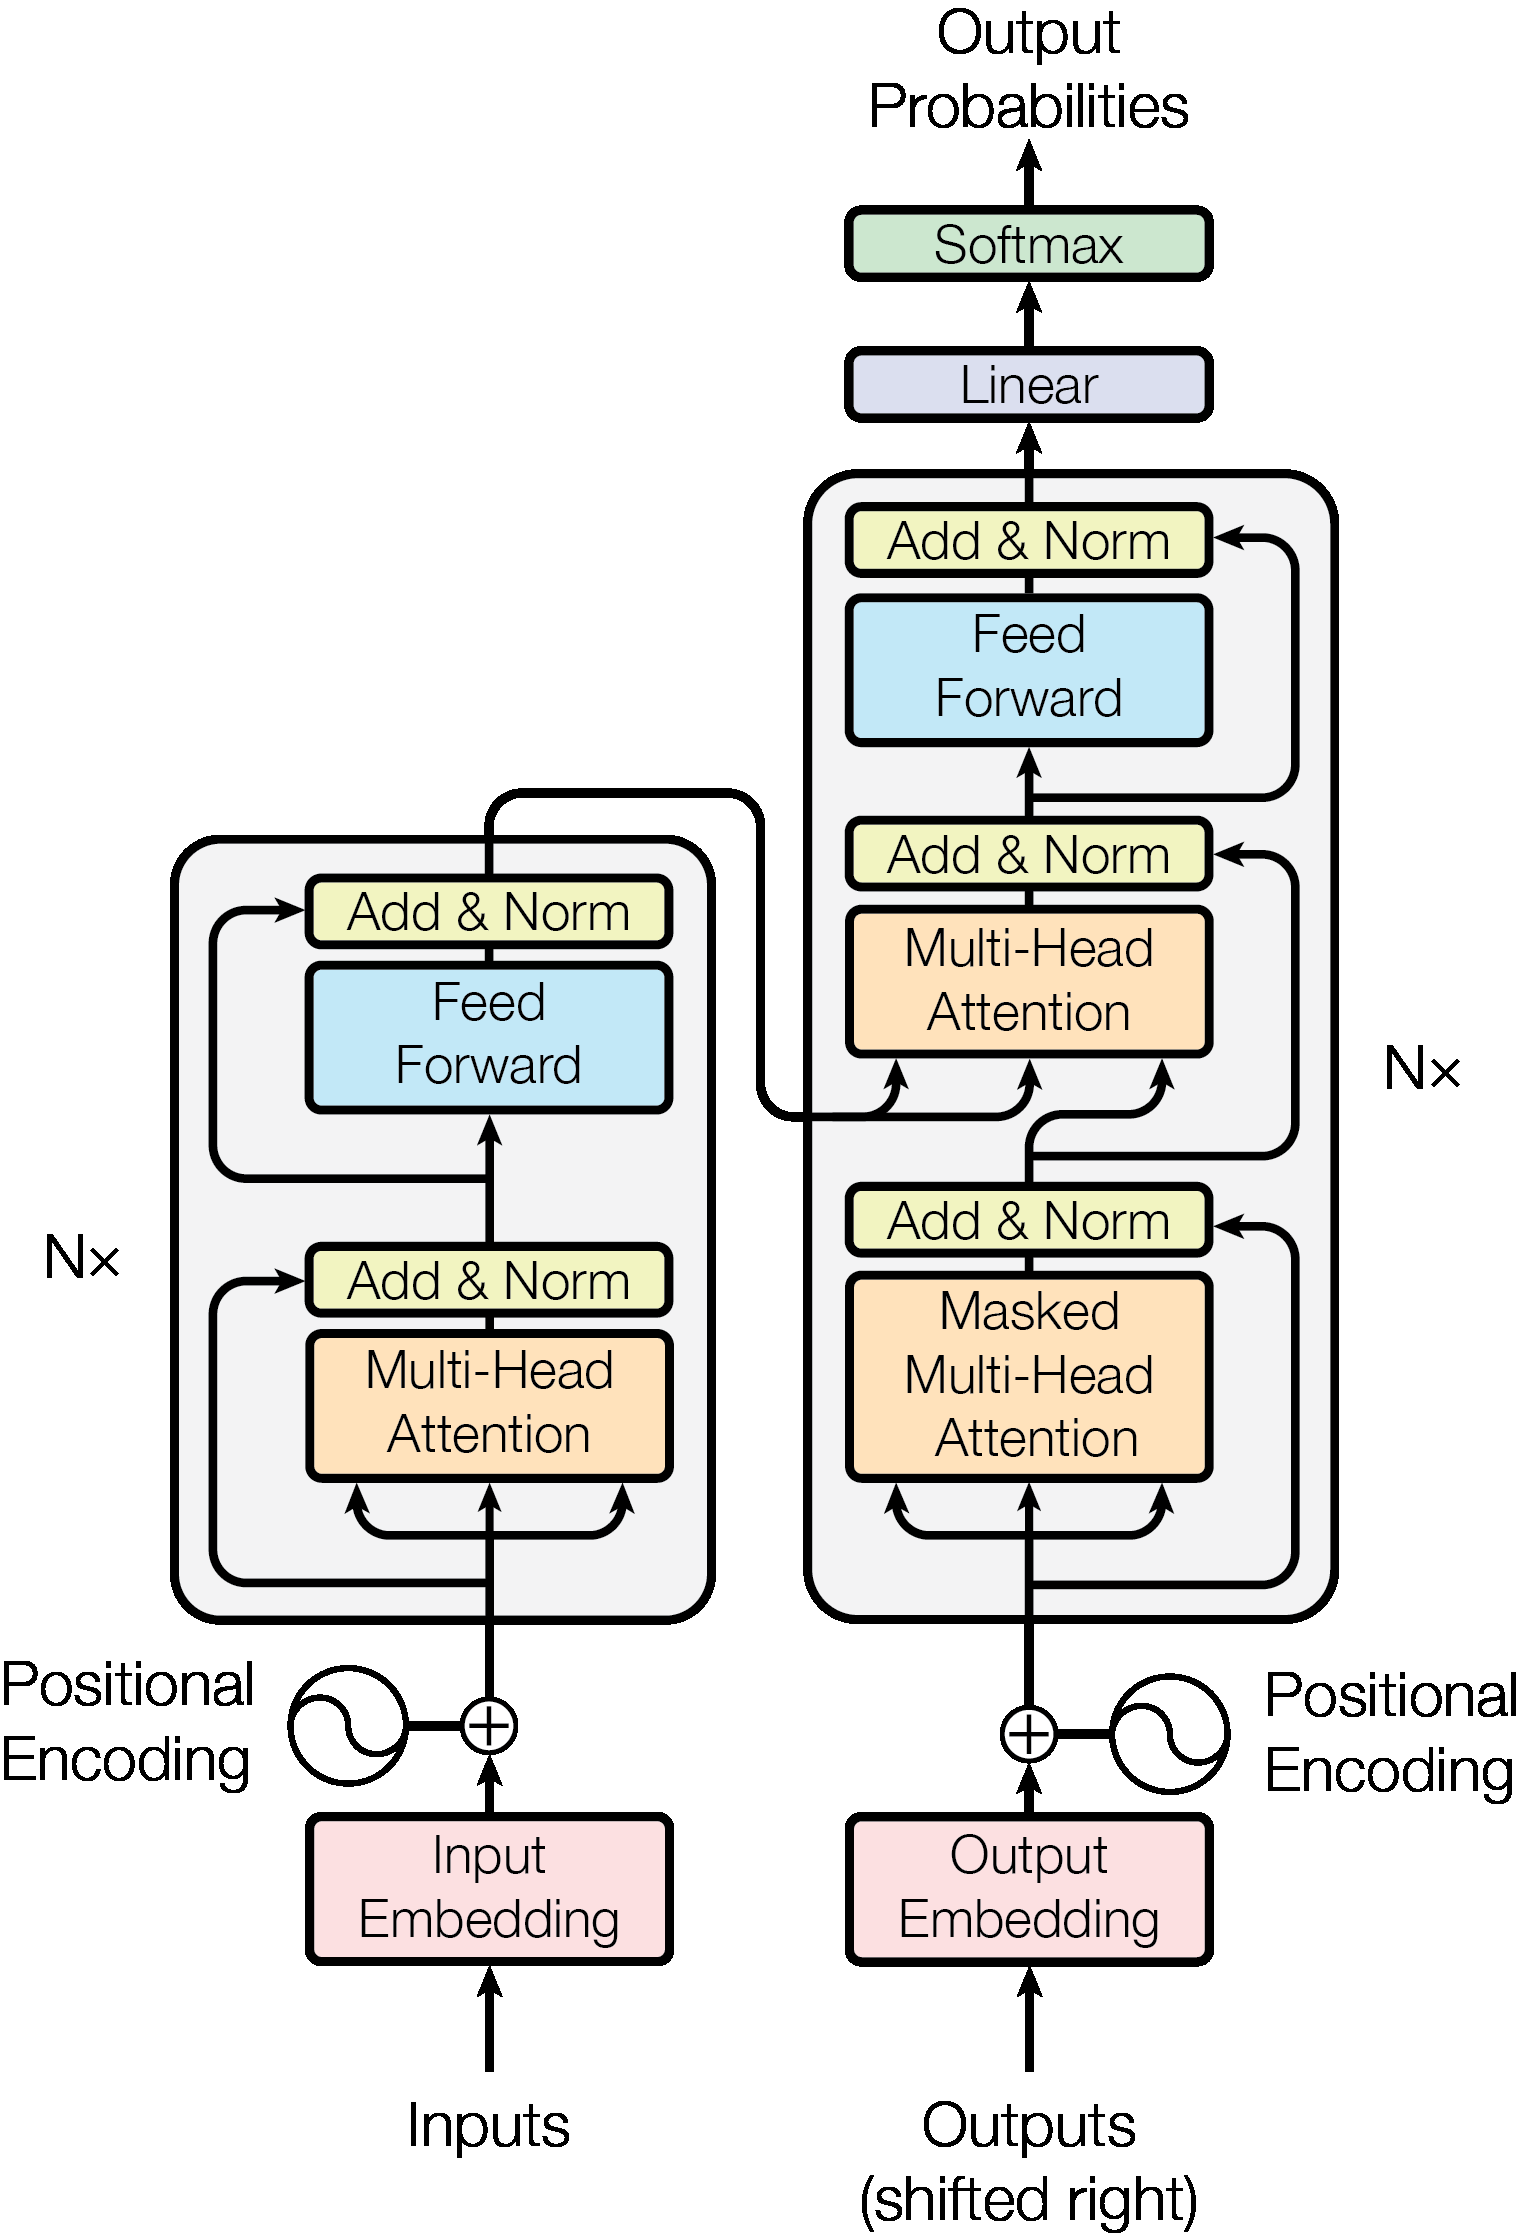
\includegraphics[width=.37\textwidth]{transformers.png}
	\caption{Transformer Architecture, from ``Attention is all you need'' \citep{attention_is_all_you_need}.}
\end{figure}

GPT models \citep{gpt} improve upon this architecture by running a supervised task-specific fine-tuning round after the unsupervised pre-training on large amount of test data.
Later models, starting from GPT-2, use zero-shot transfer learning to improve their performance \citep{gpt2}.
Zero-shot learning \citep{zeroshotlearning} trains a model to perform a task without having been explicitly trained on examples of that task; instead, it leverages knowledge gained from pre-training to infer and generalise to new tasks with the context on the prompt.

By adding only a few examples of the task at hand, a model can use few-shot learning to improve generalisation to new tasks with a limited amount of labelled data.
GPT-3 uses this to understand the structure and nature of a task with a few examples \citep{gpt3}

Despite these improvements, the models themselves are still uncalibrated and not very good at question answering \citep{how_can_we_know}.
Hallucinations are common, even for short Q\&A tasks

\subsection{Architectures of Large Language Models}
\label{llm_architectures}
\TODO{Talk about T5, Flan-T5, and Llama here.}

\subsection{Retrieval-Augmented Generation}

Large pre-trained language models store factual knowledge in their parameters.
Their ability to access this knowledge is limited, which affects their performance on knowledge-intensive tasks.

Retrieval-Augmented Generation (RAG) attempts to solve this problem by adding extra non-parametric context gathered from an index with a retriever that's trained independently \citep{rag}.
This retrieved context is fed back to the original query by adding context, which generates a combined representation which contains both the query and the original context.
An overview of this method is presented in \cref{rag_overview}.

\begin{figure}[htp]
	\centering
	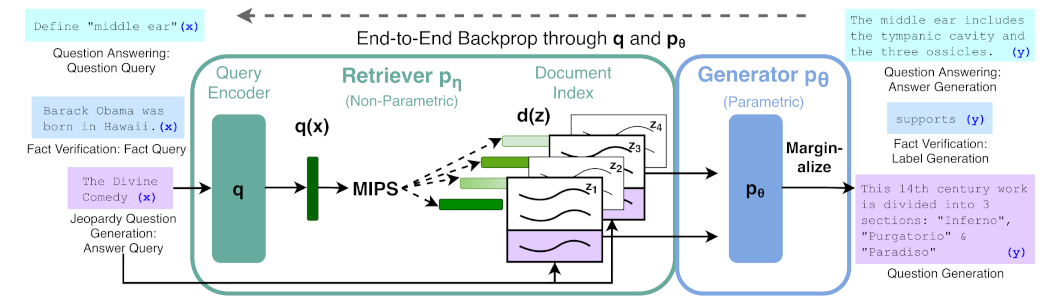
\includegraphics[width=.9\textwidth]{rag-example.png}
	\caption{An overview of the RAG approach, combining a pre-trained retriever with a pre-trained model. From ``Retrieval-Augmented Generation for Knowledge-Intensive NLP tasks'' \citep{rag}}
	\label{rag_overview}
\end{figure}

RAG can be effective in preventing hallucinations by incorporating relevant external information into the generation process, ensuring that responses are more grounded in factual data from a knowledge base.
However, this is not perfect and an even after adding a correct context the model could answer data from its internal memory.


% \begin{equation}
% 	\newcommand{\texts}[1]{\text{\tiny #1}}
% 	p_{\texts{RAG-Sequence}} \left( y \mid x \right) \approx \sum_{\mathclap{x \in \texts{top-k} \left( p \left( \cdot \mid x \right) \right)}} p_\eta \left( z \mid x \right) p_\theta \left( y \mid x, z \right) = \sum_{\mathclap{z \in \texts{top-k} \left( p \left( \cdot, \mid x \right) \right)}} p_\eta \left( z \mid x \right) \prod^N_i p_\theta \left( y_i \mid x, z, y_{1 : i - 1} \right)GA
% \end{equation}

\subsection{Knowledge Grounding on Queries with Added Context}

Knowledge grounding is the process of ensuring that information generated by a language model is consistent with a reliable external source of knowledge.
In the context of RAG-enhanced queries, this can include ensuring that answers are consistent with the knowledge in the index rather than in the model's inherent knowledge.

Various attempts have been made at understanding how good the knowledge grounding of a RAG system is, and on what is the optimal configuration of RAG.

In ``RAGGED: Towards Informed Design of Retrieval Augmented Systems'' \citep{ragged}, the authors create a framework to evaluate these systems and find that different models suit substantially varied RAG setups.
In particular, the performance of the models decreases strongly in Decoder-only models such as Llama when the context passages provides more context, while this does not happen on Seq2Seq models such as Flan.

``Characterizing Mechanisms for Factual Recall in Language Models'' \citep{factual_recall}, which is one of the main sources for this thesis, finds that when there is disagreement between the model's knowledge and the provided context then the architecture and size of the large language model will greatly affect the probability of the model choosing to use the context (which is much less prone to hallucinating) as an answer.

This paper also introduces a novel way to test this hypothesis by creating a dataset with questions and counterfactual context, an example of which is shown in \cref{query_example}.

\begin{lstlisting}[caption={Example of queries used in \citep{factual_recall}. These queries form the basis and inspiration for the dataset creation done in this thesis}, label={query_example},basicstyle=\ttfamily\small,keywordstyle=\rmfamily\bfseries,keywords={country,in,context,city},captionpos=b,frame=single,breaklines=true,xrightmargin=.15\textwidth,xleftmargin=.15\textwidth,float=h]
The capital of {country} is {in context city}
Q: What is the capital of {country}?
A:
\end{lstlisting}

By adding counterparametric information to the context, this method allows us to understand whether an answer came is parametric (that is, came from the memory of the model) or contextual (that is, came from the provided context).
